\chapter{A Novel \emph{a priori} Knowledge Driven Temporal Encoding Framework for Compressing and Recognising Pattern on Temporal Data }
\label{chap:encoding}

\section{Introduction}

%It is without a doubt that in the era of `smart' everything, availability and utility of massive volumes of digital data plays a substantial role. Historically, data was used as a part of business and gathered to serve specific needs. For example, retailers recorded sales for accounting, manufacturers recorded raw materials for quality management the number of mouse clicks on advertising banners was collected for calculating advertisement revenue and so on. But as the demand for big data analytics emerged, data no longer serves only its initial purpose. Organisations able to access huge amounts of data possess a valuable asset that when combined with the ability to analyse it, has given rise to a whole new industry.

%According to IBM \cite{data2015four}, the big data ecosystem, even though related to its earlier versions of data analytics, differs from and is characterised by the following properties:
%\begin{itemize}
%	\item Volume: This is the main characteristic of 'big data'. It is predicted that the sheer volume of data will surpass 40 zetabytes by 2020, which is a $300$ times increase from 2005 \cite{data2015four}. In the past decade, organisations have begun to store and digitise multitude of data which is leading to the exponential rise of the digital data volume. Big data technologies aims to handle such rapidly growing volume of data and deliver actionable insights from analysing such data within a time frame.   
	
%	\item Variety: This is another important property of 'big data'. Variety is associated with the availability of diverse data sources with varying properties. Variety is one the most interesting developments in technology as more and more information is digitised. Earlier due to the structured nature of data, things fit neatly in relational databases. However, with variety in the data, the lack of structure in multi-source data has a major impact on the development of big data technologies. Structured data is augmented by unstructured data, which is where things like twitter feeds, audio files, MRI images, web pages, web logs are put, anything that can be captured and stored but does not have a meta model that neatly defines it.  
	
%	\item Velocity: Velocity relates to the frequency with which a data source streams the data and also the frequency with which analytics in 'big data' environment should be able to process the data. With the rise of IoT devices and technology there has been a substantial growth in streaming data. For example, New York stock exchange streams $\approx 1$ TB of trade information every session \cite{data2015four}, modern cars have more than $100$ sensors that continuously streams high velocity data. As a result, the 'big data' technologies focus on high speed analytics that allows for actionable insight delivery.  
%\end{itemize}

Traditionally, data analytics, especially, predictive analytics and machine learning have focused on computer intensive approaches that are intended to be applied directly to the raw data present in the continuous space \citep{bishop2006pattern}. These methods aim to take advantage of the flexibility entailed by continuous mathematics (uncountable sets) to build complex learning theories that can perform pattern recognition in data. However, with the rise of big data, the machine learning technologies are dealing with new challenges with respect to real time processing of massive volumes of data. Although the machine learning community has continuously striven to learn from massive volumes of data, the development has been grounded on the assumption that the computation fits into the memory seamlessly. In contrast, the current data size has grown to such a scale that the data are becoming harder to store. 

\section{Data Compression and Inspirations from Neural Coding}
In this Chapter, the focus will be on the inspirations from the human brain that allows us to see the problem of data processing and predictive analytics problem under the big data environment from an alternate perspective. It can be observed that the continuous incoming stimuli in various forms and frequencies processed by the human brain can indeed be characterised by the properties of big data, \emph{i.e.}, volume, variety and velocity. The human brain is considered to be the most resourceful and efficient system which can recognise distinct patterns in the streaming continuous stimuli (volume) captured by multiple sensory organs (variety) in millisecond resolution (velocity). It is also observed that human brain cells, when presented with external stimuli, propagates the signal economically, over long distances using electrical impulses or spikes via the synaptic action potentials. Hence, it is imperative that there exists an efficient system, which converts the massive volume of continuous signal to discrete events or spikes. In neurobiology, the process of such analog to digital signal transformation is known as neural encoding \citep{brown2004multiple}. It is intriguing that the process of neural encoding not only converts the big streaming continuous data space into a compressed space of spikes, but the brain cells also recognise patterns in such a compressed space. The biological organisation of the brain tends to create signals with a very specific class of distributions, and it is from the perspective of evolutionary understanding that these distributions are optimised for fast analysis. The most popular hypothesis states that the signal strengths are encoded by the mean firing rate, \emph{i.e.} stronger input signal produces larger volumes of neuronal firing on an average in the brain. A range of studies \citep{mainen1995reliability, maunsell1992visual} across multiple species in the sensory and motor-neuronal system supports the validity of the mean firing rate hypothesis. A major drawback of this theory, however, lies in the association of information density with spike density. Determining the spike density in millisecond resolution from a large volume of spikes leads to a level of computational inefficiency. As per an alternate theory on neural encoding, neurons carry information in the precise timing of the spikes. This is known as the temporal encoding or spike-time encoding. Numerous research \citep{gollisch2008rapid,hallock2006temporal} has shown the presence of temporal encoding in different parts of the human brain. Temporal encoding supports the efficient representation of information that is required for very fast processing (in millisecond scale) of the stimulus presented to the human brain. As opposed to the rate coding scheme, high fluctuations in mean firing rate, also known as inter-spike interval (ISI) probability distribution is considered to be informative rather than noise in this scheme. The temporal spike-time representation of the data acts as a lossy compression of information. Most forms of learning, though, could be seen as forms of data compression. In fact, one can, in terms of pattern recognition, only learn something from data when there is redundancy in the data. In many data analysis tasks, the data is preprocessed or recoded in a way that could be seen as a form of data compression. If such preprocessing does not destroy the patterns of interest, it results in a comparative performance of the learning algorithms. The motivation of the temporal encoding, thus, in this context is to reduce large volumes of data into a compressed state with minimal loss and the maximal presence of discriminable information. Examples of data sources where such encoding is useful are high-frequency streaming data, such as the pulsar data in radio astronomy, and seismic activity data. 

\subsection{Information Theory and Data Compression}

From the viewpoint of computational theory, the data encoding problem relates to the concepts of information theory. In the seminal work on information theory, \citet{shannon2001mathematical} proposed a mathematically complete theory to quantify transmission of information in a communication channel. A conclusive finding that the amount of information in any object can be estimated as the description length of the object continues to set the stage for the development of communications and data processing. Shannon's information theory is built on a presupposition that the computable information in an object is the characteristic of a random source with known probability distribution of which the object is a part. To realise this idea, Shannon derived the `entropy' from the first principle of the theory, which is the measure of average information emitted by an object when observed. It can be described as the functional mapping of the random variable to a real number. \citet{kolmogorov1965three}, later proposed an alternate and more generalisable notion of information measurement known as algorithmic information theory. Contrary to Shannon's theory, Kolmogorov's theory of complexity \citep{kolmogorov1965three, chaitin1966length} considers information as the property of an object in isolation, irrespective of the way the object came into existence \citep{grunwald2004shannon}. It describes information as the minimum number of bits from which a message or a file can effectively be reconstructed, \emph{i.e.} the minimum number of bits suffice to store a reproducible file. A computational neuron responsible for emitting spikes from sensory data can be regarded as a logical transmission medium responsible for broadcasting continuous information received from the data source. The two neural coding hypotheses hence can be seen and described in the light of information theory. It can be observed that the rate coding scheme adheres to Shannon's interpretation of encoding. The inherent assumption of the presence of a random source with a known probability distribution in Shannon's theory is much apposite to the mean firing rate as it relates to the frequency of spikes over time. However, the interest in efficient compression of a large volume of data by a sequence of spike-timings and using it for the purpose of pattern recognition is much more in line with Kolmogorov's notion of object representation by minimal description length using computer programs. 

\section{Literature Review on Analog to Digital Data Transformation Algorithms}
A significant amount of research has focused on using the biological realism of the SNN for information processing applications akin to traditional neural networks \citep{maass1997networks}. Under the broad umbrella of SNN, the area of data encoding has been relatively unexplored compared to neuronal dynamics, network learning behaviours and so on. Human Information Processing Research Laboratory's (Advanced Telecommunication Research Institute) artificial brain (Cellular Automata Machine Brain) project \citep{de1994artificial} used data encoding as a part of its large-scale brain-like neural architecture. Hardware accelerated implementation of spike encoding for image and video processing was performed by \citet{iakymchuk2014hardware}. The literature on the application of spike encoding on the information processing task in data science is restricted to a few algorithms, such as temporal-contrast (TC) \citep{kasabov2016evolving}, Hough spiker algorithm (HSA) \citep{hough1999spiker} and Bens spiker algorithm (BSA) \citep{schrauwen2003bsa}. HSA and BSA algorithms are event-driven in nature and can be classified under the temporal encoding paradigm where the time of occurrence of an event (spike) is considered as a unit of information. The TC algorithm, also known as AER encoding, is inspired from the human visual cochlea. The TC algorithm uses a threshold-based method to detect signal contrasts or changes \citep{kasabov2016evolving}. A user-defined or auto-generated contrast threshold determines the spike events in the TC algorithm. The HSA and BSA algorithm, however, determine a spike event using a deconvolution operation between the observed signal and a predefined filter. The HSA method which is based on convolution function produces a biased converted signal where it always stays below the original waveform and this would yield an error. The BSA method on the other hand uses the Finite Impulse Response (FIR)
reconstruction filter. Even though BSA reduces the error in the HSA method and has less optimal threshold sensitivity, this method like HSA, needed a suitable filter for every type of input. Finding this filter automatically for each image would require a tremendous amount of work and time. There are some LIF neural network modelling approaches that for analog to digital transformation applied to computer vision \citep{van1998face}. These methods, however, require a large number of input neurons. 

\section{A General Framework of Spike-time Encoding and Compression for Temporal Data Sequences}
\label{sec:general}

The temporal encoding problem for pattern recognition can be formalised as a data compression problem. An encoder is hence defined as the map $\displaystyle E:\mathbb{R}^T\rightarrow\mathbf{t}^f$, where the encoder $\displaystyle E(\cdot)$ release spikes at firing times $\displaystyle \mathbf{t}^f:=\{t_1^f, t_2^f,\cdots t_n^f|t_i\in \mathbb{I}^+\}$. The temporal encoding algorithm primarily assumes that the discriminatory information is encoded by the sequence of discrete spike-timings rather than the magnitude and/or the spike density. As a consequence of this assumption, the temporal encoding aims at joint maximisation of information representation and minimisation of the spike density. Thus, it is in sharp contrast to the rate coding hypothesis. Next, the proposed \emph{a priori} knowledge driven generalised framework for temporal encoding will be presented. This framework will be further extended to formalise a temporal encoding algorithm for fMRI data.

\subsection{Formalisation of the \emph{a priori} Knowledge Driven Optimisation Problem for Data Encoding}
If one assumes a continuous source signal is represented by $ \mathbf{s}\in \mathbb{R}^T$ representing a vector of continuous values, an encoded data or a spike-train is represented by $\mathbf{b}\in \{0, 1\}^T$ as a fixed-length binary sequence. This formalisation is slightly modified from the variable length sequence formalisation of spike-timings $\{t_1^f, t_2^f,\cdots t_n^f|t_i\in \mathbb{I}^+\}$ defined earlier without any loss of generality. For example, a historical spike sequence $[01001011]$ can be rewritten as a sequence of spike-time indices $t^f :=\{1, 4, 6, 7\}$. $T$ denotes the length of the temporal signal to be encoded into spikes. The \emph{a priori} knowledge driven optimisation based encoding framework is built on the premise that 
\begin{itemize}
	\item The universal data encoder is non-existent.
	\item \emph{a priori} knowledge about the data generation process or in other words, prior knowledge of the properties of the data generation source can be injected into a predictive system that can generate a predicted signal $\mathbf{\hat{s}}$. 
\end{itemize}
For example, the fMRI data generation process behaves like a linear time invariant system, where a spike in the brain cell gives rise to a signal mimicking the gamma distribution function \citep{ashby2011statistical}, whereas the process of EEG data generation can be modelled as a phase varying mixture model of sinusoidal waves or multi-source Gaussian noise model \citep{nunezm2016eeg}. The notion of knowledge injection is further elaborated in Section \ref{sec:fmri} using fMRI as an example. If it is possible to formalise a decompression function $\mathbf{\hat{s}}$ from the spike sequence $\mathbf{b}$, the optimal encoding of data can be formulated as an optimisation problem that minimises the discrepancy between the predicted and the original signal. One way of realising such a discrepancy is by minimising the root mean squared error (RMSE) of decompression between the observed signal $s$ and the predicted signal $\mathbf{\hat{s}}:=f(\mathbf{b}, \mathbf{\Theta})$, $\mathbf{\Theta}$ being the set of additional parameters required along with $\mathbf{b}$ to describe the prediction function. The optimisation problem can be formulated as:
\begin{equation}
\begin{matrix}
\displaystyle \min_{\mathbf{b},\mathbf{\Theta}} &  \displaystyle \sqrt{\frac{\sum_t(s_t-\hat{s}(b_t,\mathbf{\Theta}))^2}{t}} \\
\textrm{s.t.} & \displaystyle b_t:=\mathbb{I}^+ \\
& \displaystyle 0\leq b_t\leq 1\\ 
& \displaystyle \sum_t b_t\leq \alpha  \\
& \displaystyle \boldsymbol{\beta}\leq \boldsymbol{\Theta} < \boldsymbol{\gamma} \\ 
\end{matrix}
\label{eq:opt}
\end{equation}

The above optimiser solves for the RMSE, subject to the following constraints:
\begin{enumerate}
	\item Binary constraints for spikes: The binary constraint for the spikes are implemented by forcing $B_t$ to be an integer and within a range of $[0, 1]$.
	\item Constraint on the number of spikes: The $\sum_t B_t\leq \alpha$ constraint enforces the maximum number of spikes to be limited to $a$. This constraint is of major importance from a biological plausibility perspective. Since the encoding scheme discussed here, aims to mimic the temporal coding behaviour of the human brain, it is always preferable to encode maximal information with the minimal number of spike.  
	\item Bounds can be set on the other parameters $\Theta$ to be optimised as part of the prediction model $f(\mathbf{B, \Theta})$.
\end{enumerate}

\subsubsection{Mixed Integer Optimisation and Genetic Algorithms}
The aforementioned optimisation problem is one related to mixed-integer programming optimisation. A mixed integer programming problem is an optimisation problem, linear or nonlinear, with or without constraints, in which some or all decision variables are restricted to have integer values. Such problems frequently arise in various application fields such as process industry, finance, engineering design, management science and others. 

Several classical computational techniques (such as, branch and bound technique, cutting planes technique, and outer approximation technique), which are reasonably efficient, have been proposed in the literature for solving mixed integer programming problems \citep{cooper1981survey, floudas1995nonlinear, grossmann2002review}. Over the last couple of decades, several stochastic algorithms have been developed and appropriately updated for problems related to mixed integer programming, such as simulated annealing, differential evolution and ant colony optimisation \citep{dorigo1996ant, babu2003differential, yiqing2007improved}. However, algorithms of this class generally harbour the capacity to provide near global optimal solutions, although the quality of the obtained solution is unstable and requires large amount of computation time.

Genetic algorithms (GA) are general purpose population based stochastic search methods inspired by Charles Darwin's principles of natural selection and genetics. \citet{holland1992adaptation} introduced the concept of GA, and it was used by \citet{kenneth1975analysis} to solve the optimisation problem. \citet{goldberg1989genetic} presents a detailed implementation of GA. To describe it in a simple manner, GA searches for sets of better solutions in the global search space. Potential solutions termed as chromosomes (individuals) are evolved iteratively over generations using a set of genetic operators such as selection, crossover and mutation. The quality of a solution or a population is measured by a fitness function, which is equivalent to a loss function in the field of machine learning and objective function in optimisation. The fitness function is responsible for evaluating how `fit' a chromosome is for reproduction. The selection operator chooses the best `fit' chromosomes for reproduction. In the reproduction process, new chromosomes are created by crossover and mutation operations. The Crossover operator blends the genetic information between chromosomes to explore the search space, whereas the mutation operator is used to maintain adequate diversity in the population of chromosomes to avoid premature convergence. The way the variables are coded into the chromosome is clearly essential for GAs' efficiency. Real coded genetic algorithms (RCGAs), which use real numbers for encoding, have fast convergence towards optima as compared to binary and Gray coded GAs \citep{deb2001multi,}. Also, `RCGAs' overcome the difficulty of Hamming Cliff
as in binary coded GAs. In the case of integer and mixed integer programming problems, many applications of GAs are available in the literature, some of which use binary coded representation \citep{cheung1997coupling, luo2001hybrid,hua2006effective} and some use real coded representations \citep{li1996nonlinear, yokota1996genetic, maiti2006application}.

Integer programming with GA modifies the vanilla GA algorithm in several ways:
\begin{enumerate}
	\item It requires custom creation, crossover and mutation function in order to enforce the variables to be integers (see \citep{deep2009real} for detail).
	\item The genetic algorithm attempts to minimise a penalty function, not the fitness function. The penalty function includes a term for infeasibility. This penalty function is combined with binary tournament selection to select individuals for subsequent generations. The penalty function value of a member of a population is:
		\begin{itemize}
			\item If the member is feasible, the penalty function is the fitness function.
			\item If the member is infeasible, the penalty function is the maximum fitness function among feasible members of the population, plus a sum of the constraint violations of the (infeasible) point. For details of the penalty function, see \citep{deb2000efficient}.
		\end{itemize}
	\item GA  does not enforce linear constraints when there are integer constraints. Instead, it incorporates linear constraint violations into the penalty function.
\end{enumerate}

In the present implementation, the mixed integer genetic algorithm solver \citep{deb2000efficient,deep2009real} was used. The constraints in \equationname \ref{eq:opt} are imposed on the parameters of $\hat{s}$. The first and second constraints are used to reduce the search space of the possible values of $b_t$ to $\{0, 1\}$. The hyperparameter $\alpha$ is used to control the maximum number of spikes and hence the spike density in the optimal solution. The other sets of hyper-parameters $\{\boldsymbol{\beta}, \boldsymbol{\gamma}\}$ are used to control the upper and lower bounds of the model parameter $\boldsymbol{\Theta}$. 

The formulation above for the proposed framework for data encoding is generic, flexible and is driven by knowledge-injection from the data source. The knowledge-injection component allows the further inclusion of systematic noise as part of $\mathbf{\hat{s}}$, if present. Examples of the inclusion of noise models, such as acoustic noise as part of linear time invariant models of fMRI are treated in \citep{sierra2008acoustic, cho1997analysis}. The hypothesis is that a sufficiently good choice of $\mathbf{\hat{s}}(\mathbf{b}, \mathbf{\Theta})$ preserves, in some cases, enhances the discriminative property of the data in a greatly compressed space. It must also be noted that this formulation adheres to the concept of the non-existence of a universal compression algorithm for all the data sources. The general framework described above can be used to derive specific methods for encoding of special types of data for which \emph{a priori} knowledge is available. One such case is fMRI data based on blood-oxygen level dependent response (BOLD). This is further introduced and illustrated in Section \ref{sec:fmri}. 

\section{GAGamma: A Spike-time Encoding and Compression Method for fMRI Data}
\label{sec:fmri}

This Section will formalise a sample prediction model $f(\mathbf{B, \Theta})$ for functional Magnetic Resonance Imaging (fMRI) data, and will present experimental results and evaluation of data encoding by solving \equationname \ref{eq:opt}.

\subsection{fMRI As a Linear Time Invariant System}

Functional magnetic resonance imaging (fMRI) is a form of magnetic resonance imaging that takes advantage of magnetic susceptibility artefacts caused by the deoxygenated haemoglobin in the brain. Magnetic susceptibility measures the magnetic properties of the interaction between a tissue or other substance and the in-scanner magnetic field strength. Magnetically susceptible materials distort the homogeneity of a magnetic field: materials with negative magnetic susceptibility are known as diamagnetic, and those with positive magnetic susceptibility are referred to as paramagnetic. Introduction of a paramagnetic substance such as deoxyhaemoglobin into the scanner magnetic field causes variability in field strength, spin dephasing, geometric distortion and loss of signal; fMRI exploits this property by measuring changes in the relative ratio of oxygenated (diamagnetic) to deoxygenated (paramagnetic) haemoglobin in the blood.

Functional Magnetic Resonance Imaging (fMRI) is most commonly acquired using Blood Oxygen Level Dependent (BOLD) response. The BOLD response is measured by the changes in deoxyhaemoglobin at time $t$, and is caused by neural activation in the brain. The neural activations are caused by some sequence of events driven by the task performed by the subject \citep{friston1995analysis}. The BOLD response is mathematically described as a time invariant system, \emph{i.e.} a system whose output does not depend explicitly on time. Under the appropriate experimental protocol, BOLD response also pertain to the superposition principle and henceforth can be designed as a linear time invariant (LTI) \citep{vazquez1998nonlinear}. According to \citet{chen1995linear}, a LTI system is said to be completely characterised by convolution integral functions. The fMRI BOLD is described by the convolution of the spikes $\mathbf{b}$ and the haemodynamic response function (HRF), $h(\mathbf{\Theta})$. This operation is characterised by \equationnames \ref{eq:conv1} and \ref{eq:conv2}. 

\begin{equation}
\label{eq:conv1}
\displaystyle \mathbf{\hat{s}}:=\int_0^t \mathbf{b}(\tau)h(t-\tau)d\tau
\end{equation}

\begin{equation}
\label{eq:conv2}
\displaystyle \mathbf{\hat{s}}(\mathbf{b}, \mathbf{\Theta}):=\mathbf{b}\ast h(\mathbf{\Theta})
\end{equation}

\begin{equation}
\label{eq:hrf}
h(\theta_1, \theta_2):=\frac{1}{\theta_2^{\theta_1}\mathcal{T}(\theta_1)}t^{\theta_1-1}e^{-\frac{t}{\theta_2}}
\end{equation}
\subsection{GAGamma Optimisation Problem for fMRI}
Numerous models for HRF have been proposed in the literature \citep{boynton1996linear,friston1998nonlinear,glover1999deconvolution}. The majority of mathematical models for the canonical HRF are found to be some variant of the gamma function. In all the experiments performed here, the gamma distribution function has been used as the HRF model (\equationname \ref{eq:hrf}). This function is characterised by the parameter set $\displaystyle \mathbf{\Theta}:=\{\theta_1, \theta_2\}$, where $\theta_1\in \mathbb{R^+}$ and $\theta_2\in \mathbb{R^+}$ controls the shape and the scale of the gamma function respectively. By substituting \equationnames \ref{eq:conv2} and \ref{eq:hrf} in \equationname \ref{eq:opt}, the encoding problem can be reduced to solving \equationname \ref{eq:gagamma} and is referred to as GAGamma encoding algorithm hereafter.

\begin{equation}
\begin{matrix}
\displaystyle \min_{\mathbf{b},\theta_1, \theta_2} &  \displaystyle \sqrt{\frac{\sum_t(s_t-\hat{s}(b_t,\theta_1, \theta_2))^2}{t}} \\
\textrm{s.t.} & \displaystyle b_t:=\mathbb{I}^+ \\
& \displaystyle 0\leq b_t\leq 1\\ 
& \displaystyle \sum_t b_t\leq \alpha  \\
& \displaystyle \beta_1\leq \theta_1\leq \gamma_1 \\ 
& \displaystyle \beta_2\leq \theta_2\leq \gamma_2 \\

\textrm{where} & \displaystyle \hat{s}_t(b_t,\theta_1,\theta_2):=b_t\ast \frac{1}{\theta_2^{\theta_1}\mathcal{T}(\theta_1)}t^{\theta_1-1}e^{-\frac{t}{\theta_2}}
\end{matrix}
\label{eq:gagamma}
\end{equation}

\subsection{Distinction of GAGamma from HSA and BSA}

At this point, it is imperative to make the distinction between the GAGamma and the existing HSA and BSA algorithms. Apart from exhibiting similarities in convolution framework, HSA and BSA also resemble GAGamma as methods of stimulus estimation using FIR. Nevertheless, the data encoding approach in HSA and BSA use a deconvolution (of \equationname \ref{eq:conv1}) approach contrary to the optimisation approach in GAGamma. The knowledge-injection component of GAGamma, as part of formalisation of $\mathbf{\hat{s}}$ and the optimisation approach, has two distinct benefits over the deconvolution-based methods: 
\begin{itemize}
	\item A generic Gamma function has been used as the knowledge-injection component to $\mathbf{\hat{s}}$ in GAGamma, which is driven by the existing knowledge about the fMRI data as opposed to the generic sinusoidal function used as the FIR in BSA. It is also argued that this formulation allows the inclusion of additional knowledge about the data source (such as systematic noise) if present, providing greater flexibility in the formulation of the encoding algorithm.
	
	\item The optimisation problem formulation in GAGamma jointly optimises for the parameter set $\mathbf{\Theta}$ and $\mathbf{b}$. This formulation thus includes the parameter set $\mathbf{\Theta}$ of the prediction model $\mathbf{\hat{s}}$ and the spike sequence $\mathbf{b}$ for each individual voxel or feature. In HSA and BSA, the equivalent filter parameters are predetermined for the whole set of voxels and are not learned from the data.
	
	\item The constraint $\everymath{\displaystyle} \sum_t b_t\leq \alpha$ in GAGamma ensures the flexibility in choosing the desired spike density, hence the ability to control the compression and quality of signal reconstruction. The BSA or HSA algorithm, on the contrary, accommodates no such control in the encoding framework.        
\end{itemize}

\section{Experiments and Evaluation}
\subsection{Description of Dataset}
The experiments described in this Chapter were performed on the publicly available benchmark Starplus fMRI dataset \citep{mitchell2001starplus} collected by The Centre for Cognitive Brain Imaging, Carnegie Mellon University. The Starplus experiment was conducted on a set of $7$ subjects. Each subject had undergone multiple trials of exactly the same cognitive experiment. At every trial lasting for $27$ seconds, a set of stimuli were presented to a subject in the following order:
\begin{enumerate}
	\item The first stimulus (picture or sentence) was presented at the beginning for 4 seconds.
	\item A blank screen was presented during the interval of $5-8$ seconds.
	\item The second stimulus (sentence or picture) was presented during the interval of $9-12$ seconds.
	\item A rest period of $15$ seconds was added after the presentation of the second stimulus.
\end{enumerate}
While the subject performed the cognitive tasks, fMRI images from specific regions of interest (ROI) of the brain were collected at every $500$ms interval. The preprocessed fMRI dataset has been used in a number of pattern recognition studies \citep{mitchell2003classifying, mitchell2008predicting, shinkareva2008using}. In this study, this benchmark dataset was chosen to build pattern recognition systems that can predict and discriminate between the binary cognitive states of a subject `seeing a picture' and `reading a sentence'. Two subjects were chosen (id: 04847 and 07510) randomly and two spatial ROIs; Calcarine Sulcus (`CALC') and Left Intra-Parietal Sulcus (`LIPL') were used for the experiments. The choice of the ROI is based on previous work \citep{do2014robust} that found these ROIs to be amongst the most discriminatory in the raw continuous data space. The dataset for each subject is composed of $40$ samples (trials) of each class, and each sample is made up of $452$ and $483$ voxels in subject 04847 and 07510 respectively. Each cognitive task lasted for a total of $8$ seconds emitting $16$ fMRI images for each class within a trial.

\subsection{Evaluation Metrics}

Three metrics have been used to evaluate and compare the performance of the encoding techniques and the traditional `no-encoding' (raw data) approach. The evaluation criteria and the baseline encoding techniques are elaborated below:

\subsubsection{Bit Compression Ratio} 
The Bit Compression Ratio (BCR) is defined as the ratio between the average number of bits required to store an encoded dataset and the number of bits required to store a raw dataset, respectively. BCR is directly associated with the relative description lengths (DL) and data type of the datasets. The DL of a dataset is described by the length of the dataset represented by the number of values in the dataset. If one assumes a dataset intended for pattern recognition is represented by $D_{raw}:=\{x_1, x_2, \cdots x_n| type(x_i)=\mathbb{R}\}$ which is transformed by an encoding algorithm to $D_{encoded}:=\{y_1, y_2, \cdots y_m| type(y_j)=\mathbb{I}^+\}$, where $m$ and $n$ are the DL of the raw and the encoded data respectively. The BCR is then estimated as:
\begin{equation}
	BCR:=\frac{m\times sizeof(\mathbb{I}^+)}{n\times sizeof(\mathbb{R})}
\label{eq:compression}
\end{equation}  
The notion of BCR (\equationname \ref{eq:compression}) can be analysed from the viewpoint of the Kolmogorov complexity. As described earlier, Kolmogorov's descriptional complexity aims at a simpler object representation and simplicity is measured by the DL of the object. Here, the object being a pattern recognition dataset, the objective is to achieve simpler representation of the dataset by performing the encoding operation. This is achieved by minimising the numerator $m\times sizeof(\mathbb{I}^+)$. A compression is said to be achieved, if $0<BCR<1$ is satisfied. It is also quite evident from \equationname \ref{eq:compression} that the data type of the objects present in the dataset contributes significantly to the BCR metric. In this case, the encoded data being represented by positive integers (spike-timings) as opposed to the floating-point numbers in the raw data, already contribute significantly to BCR. Additionally, the temporal encoding algorithms aspire to minimise the DL of the object ($m<<n$), thus achieving a lower BCR.            
	
\subsubsection{Decoding Error} The decoding error metric is the measure of the decompression reliability, \emph{i.e.} the ability to recover the original signal from the compressed spike-timings reliably. RMSE of signal reconstruction between the original signal $s$, and the predicted signal $\hat{s}$ has been used as a measure of decompression reliability in this study. The RMSE is given by:
\begin{equation}
	\displaystyle RMSE:= \sqrt{\frac{\sum_t(s-\hat{s}(b_t,\Theta))^2}{t}}
\end{equation}
A low RMSE of the signal reconstruction indicates higher preservation of the original data in the spike-timings. However, low RMSE is not necessarily indicative of a better encoding for pattern recognition. For example, an encoder producing better reconstruction error for noisy data may indicate inefficient noise filtering. It must also be noted that the prediction models are built on the spike-time data and have no knowledge of the mapping $\mathbf{s}\rightarrow \mathbf{b}$ being performed beforehand. Hence, although this metric plays an important role in evaluating the robustness of the encoding algorithm with respect to the reconstruction of the raw data, the effect on the quality of pattern recognition performance is unaffected.
	
\subsubsection{Classification Performance} From the pattern recognition viewpoint, due to the balanced nature of the dataset, the classification accuracy is the most important and relevant measure of success and this has been used as a measure of classification performance. The mean accuracy is estimated from thirty independent runs of 50/50 train/test split of the binary classification data described previously. 

As the data that was encoded was intended to be used for pattern recognition problems, conservation and possible enhancement of the discriminatory information in the spike-timings is as crucial as efficient compression of the data. This is a distinctly different approach from the existing ones in pattern recognition. In the traditional pattern recognition approach, the volume of the data plays a crucial role in the performance of the pattern recognition algorithms to produce accurate predictions. In the temporal encoding approach, by keeping both compressibility and classification performance as the criteria of evaluation, the aim is to benefit from the efficient representation of information in the data along with the classification performance. It is, thus, important to have a balance between compression and conservation of discriminatory information in the encoded data. 

\subsection{Design of Experiments}
\begin{figure}
	\centering
	\includegraphics[width=\linewidth]{fig/encoding/flowchart.png}
	\caption{Flowchart depicting the evaluation criteria and experimental protocol used in this research.}
	\label{fig:flowchart}
\end{figure}

\figurename \ref{fig:flowchart} shows a flowchart of the experimental design used in this Chapter. The experimental protocol begins with the raw temporal data $\mathbf{s}$. At the first step, the encoding operation is performed on $\mathbf{s}$ to generate the encoded spike-time data $\mathbf{b}$. In the second step, a K-NN based prediction model is learned using a fraction of $\mathbf{b}$. The rest of $\mathbf{b}$ is used to test the performance of the model emitting the prediction performance. The next evaluation criteria relate to the compressibility of the encoding algorithms. To evaluate the compressibility, BCR is calculated by comparing $\mathbf{b}$ and $\mathbf{s}$. Finally, the lossiness of the encoding operation is evaluated by comparing predicted signal $\hat{s}$ produced by the decoding algorithm (corresponding to the encoding algorithm) and the ground truth $s$ to emit the decoding error.   

\subsubsection{K-Nearest Neighbour (K-NN) Algorithm with Custom Distance Function}
\label{parag:knn_custom}
As discussed earlier, the non-parametric K-NN algorithm for building the classification model from the data is used. The class label prediction of a new sample (in this case a spike-train) in K-NN is a majority vote between the neighbours of the new sample, where the sample is assigned to the class label most common among its K nearest neighbours. To evaluate the neighbourhood of a sample, it is hence necessary to calculate pairwise distances between the sample to be predicted and the training samples. As the key interest is in learning about a K-NN model for both raw (in continuous space) and spike-time (discrete space) data, there have been two different distance functions used: raw and encoded data. For the raw data in the continuous space, the standard Euclidean distance or the $L^2$ norm as the distance function was used. On the other hand, for the spike-time dataset, the spike asynchronicity based distance function was used, and is described below:

\paragraph{Spike asynchronicity based distance function:} Here, I propose a distance function that can capture the relative distance between a pair of the spike-train samples. Since the concern is with using spike-timings as a carrier of information, a useful way to capture similarity between a pair of spike-train samples is to record if the two samples have spiked at the same time instances. Therefore, mean absolute asynchronicity has been used as the distance function. The mean absolute asynchronicity based distance function between two spike-train samples $\displaystyle \mathbf{b_1}\in \{0, 1\}^{T\times M}$ and $\displaystyle \mathbf{b_2}\in \{0, 1\}^{T\times M}$ is formalised as the mean pairwise Hamming distance between all feature-wise pairs $\mathbf{b_1^{m}}$ and $\mathbf{b_2^{m}}$, where $M$ is the feature count. As the spike-time data lies in the binary space, the mean pairwise Hamming distance is equivalent to the mean XOR distance between the pairs of spike sequences. 

\subsection{Baseline Encoding Algorithms}    

In this study, three different encoding methods have been compared and evaluated. It must be noted that for each encoding or compression algorithm, there is also a decoding algorithm which decompresses the spike-trains into the reconstructed signal $\mathbf{\hat{s}}$.   
\begin{algorithm}
	\begin{algorithmic}[1]
		\STATE input: $s, filter, threshold_{BSA}$
		\STATE output: $b$
		\STATE $b\Leftarrow 0$
		\STATE $L=length(s)$
		\STATE $F=length(filter)$
		\FOR{$t=1:(L-F+1)$}
			\STATE $e_1\leftarrow 0$
			\STATE $e_2\leftarrow 0$
			\FOR{$k=1:F$}
			    \STATE $e_1 \pluseq |s(t+k)-filter(k)|$
			    \STATE $e_2 \pluseq |s(t+k-1)|$      
			\ENDFOR
			\IF{$e_1\leq (e_2-threshold_{BSA})$}
			    \STATE $b(t)\leftarrow 1$
			    \FOR{$k=1:F$}
			        \STATE $s(i+j-1)\minuseq filter(k)$
			    \ENDFOR
			\ENDIF
		\ENDFOR
		\caption{BSA encoding algorithm}
		\label{alg:bsa-enc}
	\end{algorithmic}
\end{algorithm}

\begin{algorithm}
	\begin{algorithmic}[1]
		\STATE input: $b, filter$
		\STATE output: $\hat{s}$
		\STATE $L=length(b)$
		\STATE $F=length(filter)$
		\FOR{t=1:L-F+1}
		    \IF{$b(t)==1$}
		        \FOR{$k=1:F$}
		            \STATE $\hat{s}(t+k-1)\pluseq filter(k)$
		        \ENDFOR
		    \ENDIF
		\ENDFOR
		\caption{BSA decoding algorithm}
		\label{alg:bsa-dec}
	\end{algorithmic}
\end{algorithm}


\begin{itemize}
	\item GAGamma: The GAGamma encoding method is outlined and described in Section \ref{sec:fmri}. The encoding and decoding principles are given by \equationnames \ref{eq:conv2} and \ref{eq:gagamma}.
	
	\item BSA: The BSA encoding and decoding algorithms \citep{schrauwen2003bsa} are formalised in \algorithmnames \ref{alg:bsa-enc} and \ref{alg:bsa-dec}, respectively. The BSA encoding algorithm takes a filter function and a threshold value as input along with the signal $s$. The deconvolution approach of BSA begins with a FIR filter, and at every time instant $\tau$ calculates two error metrics: $\sum_{k=0}^{P}abs(s(k+\tau)-h(k))$ and $\sum_{k=0}^{P}abs(s(k+\tau)$, where $P$ is the number of filter taps. If the first error is less than the second error minus the threshold, then the BSA encoder fires a spike and subtracts the filter from the input \citep{schrauwen2003bsa}.  
	
	\item Temporal contrast: The temporal contrast algorithm captures the greater than average changes in the data as spikes. \algorithmnames \ref{alg:tc-enc} and \ref{alg:tc-dec} presents the temporal contrast encoding and decoding algorithms respectively. One major characteristic and deviation of temporal contrast algorithm from the temporal encoding framework is its ability to generate spikes with positive and negative polarity. Since the main interest is in the spike-timings, during the classification, the polarity of the spikes have been ignored. The algorithm takes the $factor\in \{0, 1\}$ parameter as input. This parameter controls the estimate of the $threshold_{TC}$ variable, which is responsible for determining the spike-timings. 
	
\end{itemize}
\begin{algorithm}
		\begin{algorithmic}[1]
			\STATE input: $s$, $factor$
			\STATE output:$b, threshold_{TC}$
			\STATE $L\leftarrow length(s)$
			\FOR {$t=1:L-1$}
			\STATE $diff\leftarrow |s(t+1)-s(t)|$
			\ENDFOR
			\STATE $threshold_{TC}\leftarrow mean(diff)+factor\cdot std(diff)$
			\STATE $diff\Leftarrow [0,diff]$
			\FOR{$t=1:L$}
			\IF{$diff(t)>threshold_{TC}$}
			\STATE $b(t)\leftarrow 1$
			\ELSIF{$diff(t)<-threshold_{TC}$}
			\STATE $b(t)\leftarrow -1$
			\ELSE
			\STATE $b(t)\leftarrow 0$
			\ENDIF
			\ENDFOR
			\caption{Temporal contrast encoding algorithm}
			\label{alg:tc-enc}
		\end{algorithmic}
	\end{algorithm}

	\begin{algorithm}
		\begin{algorithmic}[1]
				\STATE input: $b, threshold_{TC}$
				\STATE output: $\hat{s}$
				\STATE $\hat{s}\leftarrow 0$
				\STATE $L\leftarrow length(b)$
				\FOR {$t=2:L$}
				\IF{$\hat{s}(t)>0$}
				\STATE $\hat{s}(t)\leftarrow \hat{s}(t-1)+threshold_{TC}$
				\ELSIF{$\hat{s}(t)<0$}
				\STATE $\hat{s}(t)\leftarrow \hat{s}(t-1)-threshold_{TC}$
				\ELSE
				\STATE $\hat{s}(t)\leftarrow \hat{s}(t-1)$
				\ENDIF
				\ENDFOR
				\caption{Temporal contrast decoding algorithm}
				\label{alg:tc-dec}
		\end{algorithmic}
	\end{algorithm} 
\subsection{Results}

\begin{table}
	\centering
	\caption{Comparative evaluation of the data encoding algorithms applied to subject 04847 and 07510 in the Starplus fMRI dataset.}
	\label{tab:classification}
	\resizebox{\textwidth}{!}{%
		\begin{tabular}{@{}clcccc@{}}
			\toprule\toprule
			subject id & method & data type \footnotemark{} & BCR & decoding error & classification accuracy (K\footnotemark{}) \\ \midrule
			\multirow{5}{*}{04847} & GAGamma-16 & int & $0.15$ & $\mathbf{0.07}$ & $87.41\pm 4.80 (16)$  \\
			& GAGamma-3 & int & $\mathbf{0.04}$ & $0.29$ & $85.02 \pm 4.76 (11)$ \\
			& BSA & int & $0.08$ & $0.15$ & $84.5\pm 4.47 (3)$ \\
			& TC & int & $0.06$ & $0.23$ & $54.16\pm 5.47 (1)$ \\
			& No-encoding & decimal & $1$ & - & $\mathbf{89.55\pm 4.60} (1)$ \\\midrule
			\multirow{5}{*}{07510} & GAGamma-16 & int & $0.15$ & $\mathbf{0.06}$ & $76.00\pm 5.89 (8)$ \\
			& GAGamma-3 & int & $\mathbf{0.04}$ & $0.27$ & $\mathbf{81.16\pm 7.50} (2)$ \\
			& BSA & int & $\mathbf{0.04}$ & $0.15$ & $74.08\pm 6.71 (8)$ \\
			& TC & int & $0.05$ & $0.26$ & $52.75 \pm 5.84 (2)$ \\
			& No-encoding & decimal & $1$ & - & $79.11 \pm 3.99 (5)$ \\\midrule
			& Random & int & $0.11$ & - & $52.58\pm 4.79 (1)$ \\ \bottomrule\bottomrule
		\end{tabular}%
	}
\end{table}
For the comparative evaluation of the encoding methods with the classical `no-encoding' (raw data) method, identical experiments were performed for the subjects 04847 and 07510. For the GAGamma encoding, two sets of hyper-parameters have been used to demonstrate the tuning capability of the algorithm. In the GAGamma-16  method, the hyperparameter values $[\alpha=16, \beta=0, \gamma=10]$ (see \equationname \ref{eq:gagamma}) were used, and in the GAGamma-3 method, $[\alpha=3, \beta=0, \gamma=10]$ were used. The BSA encoding algorithm takes a finite impulse response $filter$ and a $threshold_{BSA}$ as input. In the current experiments, the low pass FIR filter of size $10$ and the $threshold_{BSA}=0.95$ have been used. These values are guided by the existing literature on the application of BSA on brain data \citep{nuntalid2011eeg}. For the temporal contrast encoding, the hyper-parameter $factor=0.6$ has been used. As a baseline, a randomly generated spike-train dataset has also been included. The random spike-time dataset was created using a Poisson's distribution function ($\lambda=0.6$). Varying the $\lambda$ parameter affects the BCR directly for random spike generation. It must be noted that the presented results are non-exhaustive in the hyperparameter space of different encoding methods. In the `no-encoding' method, the raw dataset was created by transforming each multi-dimensional time series (set of images) within a trial into a single static observation by concatenating the feature values across the $16$ time intervals similar to the approach employed by \citet{mitchell2003classifying}. 

\footnotetext[1]{An integer is assumed to take 8 bits and floating-point number 32 bits.}    
\footnotetext[2]{K: Number of nearest neighbours used in K-NN algorithm}


\subsubsection{Comparison Between `Encoding' and `No-encoding'} The advantages of performing encoding as opposed to using the raw data (`no-encoding') is well established in \tablename \ref{tab:classification}. This table shows the experiments replicated across subjects 04847 and 07510. For every subject, three temporal encoding methods were evaluated. They are the proposed GAGamma, BSA and the temporal contrast encoding. In the GAGamma-X method, $X$ corresponds to the value of the maximum number of allowed spikes, $\alpha$ (\equationname \ref{eq:gagamma}). The temporal encoding methods are compared against the raw data or the `no-encoding' method along with a random spike-train as a baseline. As discussed earlier, the encoding methods are evaluated using BCR, decoding error and classification accuracy as the measures of success. The decoding error metric is not applicable for the `random' and `no-encoding' method. This is because in `no-encoding' and `random' method, the raw data and a random spike generator were used, respectively, for pattern recognition and thus, encoding principles are not applied in these two cases. 
	
It is observed that the encoding operations could compress the data dramatically and thus attaining BCR values between $0.04$ and $0.15$ \emph{i.e.} an approximate compression of $6$ to $25$ times compared to the raw data. The most important metric of evaluation, the classification accuracy column in \tablename \ref{tab:classification}, shows that the GAGamma and BSA methods achieve comparable classification performances with respect to the `no-encoding' method, and hence can capture the discriminatory information in the spike-time data well. It should also be noted that for subject 07510, the GAGamma-3 method achieved a classification performance of $81.16\pm 7.50\%$ as opposed to the $79.11\pm 3.99\%$ by the raw data and thus outperforming the `no-encoding' method. This, it can be argued is due to the ability of the encoding algorithms to represent the information in the raw data into the spike-time and thus concisely present to the classifier.
	
\subsubsection{Comparison of the Temporal Encoding Algorithms} 

\begin{figure}
	\centering
	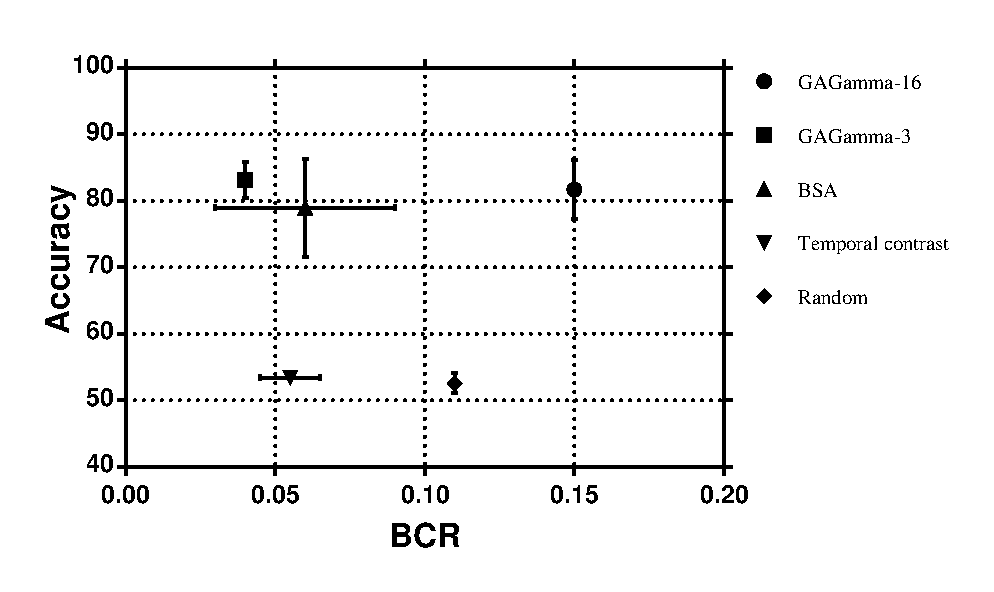
\includegraphics[width=\linewidth]{fig/encoding/encoding_comp_graph.eps}
	\caption{Plot illustrating the comparison of the quality of the encoding methods with respect to the mean classification accuracy and bit compression ratio across the two subjects. The horizontal and the vertical error bars represent the standard deviation of accuracy and BCR across experiments.}
	\label{fig:eval-chart}
\end{figure}


\figurename \ref{fig:eval-chart} graphically depicts the quality comparison of the different encoding techniques. The plot shows the mean BCR and the classification accuracy of the encoding techniques across the two subjects. The horizontal and vertical error bars are the standard deviations of the BCR and accuracy respectively. It can be initially observed that the GAGamma-16 and GAGamma-3 encodings show superior mean performance in the pattern recognition task compared to other methods. However, the aim is to simultaneously achieve high classification performance and a highly compressed information representation, and thus, the GAGamma-3 and BSA data points residing on the top left quadrant of the plot fare better overall in both respects. From the error bar representations, it can also be seen that the GAGamma method has a negligible deviation on BCR. This is due to the flexibility that the GAGamma method provides to control the spike density by the constraint $\everymath{\displaystyle} \sum_t b_t\leq \alpha$ (\equationname \ref{eq:gagamma}) without sacrificing much pattern recognition performance. This can be of significant importance, especially, for the storage and transmission of large volumes of streaming data within limited resources, where the encoding operation can precisely tune the compression rate and hence the storage. It is also recognised from the plot that the temporal contrast encoding method fares poorly in this experiment and is no better than a random spike generator.              

\begin{figure}
	\centering
	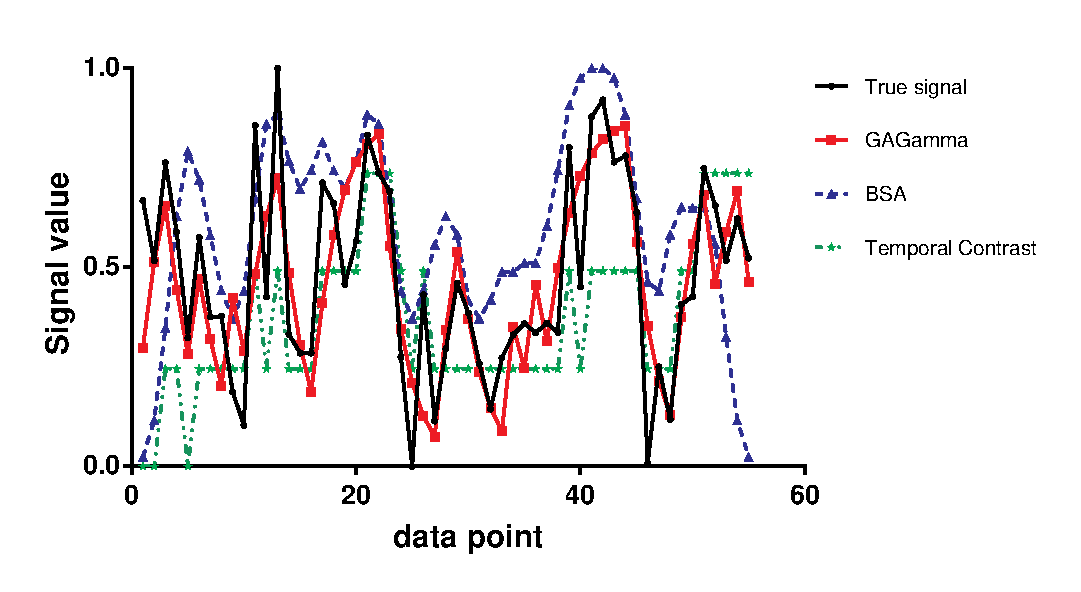
\includegraphics[scale=0.9]{fig/encoding/signal_recon.eps}
	\caption{Comparison of signal reconstruction ($\hat{s}$) from a spike sequence by GAGamma-16 decoding  algorithm (\equationname \ref{eq:conv2}), BSA decoding algorithm (\algorithmname \ref{alg:bsa-dec}) and Temporal contrast decoding algorithm (\algorithmname \ref{alg:tc-dec}). The true signal is randomly selected from subject 04847 ($10^{th}$ trial and $23^{rd}$ voxel).}
	\label{fig:recon}
\end{figure}


\begin{figure}
	\centering
	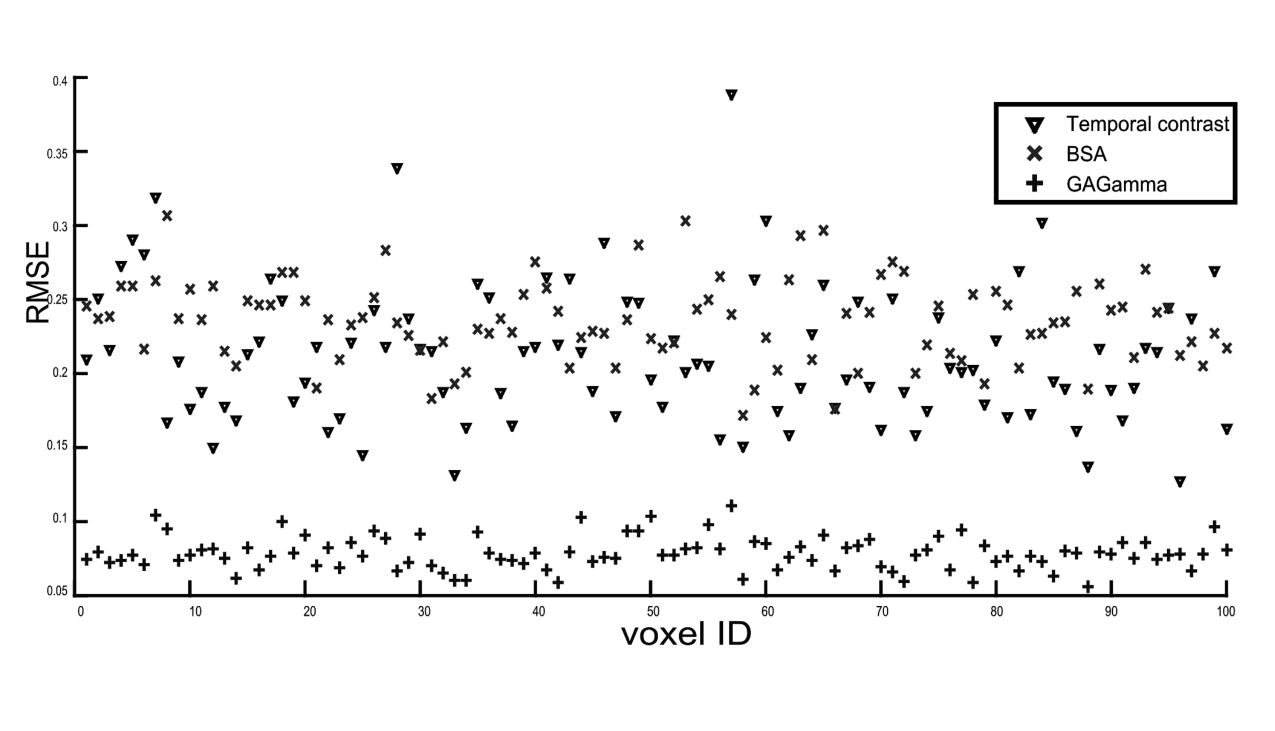
\includegraphics[width=\linewidth]{fig/encoding/recon.eps}
	\caption{Comparison of RMSE of reconstruction between GAGamma, BSA and Temporal Contrast across $100$ voxels of second trial in subject 04847.}
	\label{fig:RMSE}
\end{figure} 

\tablename \ref{tab:classification} also shows an inverse relationship between the BCR and the decoding error. This is because it requires significantly more effort to accurately represent the seasonal variations in the data using fewer spikes. However, if decoding robustness is of major importance, the GAGamma method can be tuned to maximise spike density and thus will have minimal loss in the signal reconstruction and thus sacrificing the compression. \figurename \ref{fig:recon} shows an example of the signal reconstruction done by the GAGamma-16, BSA and temporal contrast decoding algorithms. In \figurename \ref{fig:RMSE}, comparisons were also performed on the RMSE of signal reconstruction across $100$ different voxels using spikes encoded by the encoding methods. It can be clearly observed that the signal reconstruction by GAGamma (smaller RMSE means better reconstruction) is superior to the others as not only can it reconstruct the bigger trends in the signal but also the seasonal variations.

As part of the optimisation, the GA-gamma encoding method also optimises for the parameters of the response filter $H$. \figurename \ref{fig:gamma} shows the gamma haemodynamic response filters learned by the model for a single voxel across 7 trials. It can be seen from the figure, that for a single voxel across trials, the shape of the HRF is nearly consistent, but varies in the scale. This result is consistent with the notion of the existence of minor variations of HRF across voxel and/or subject.

\begin{figure}
	\centering
	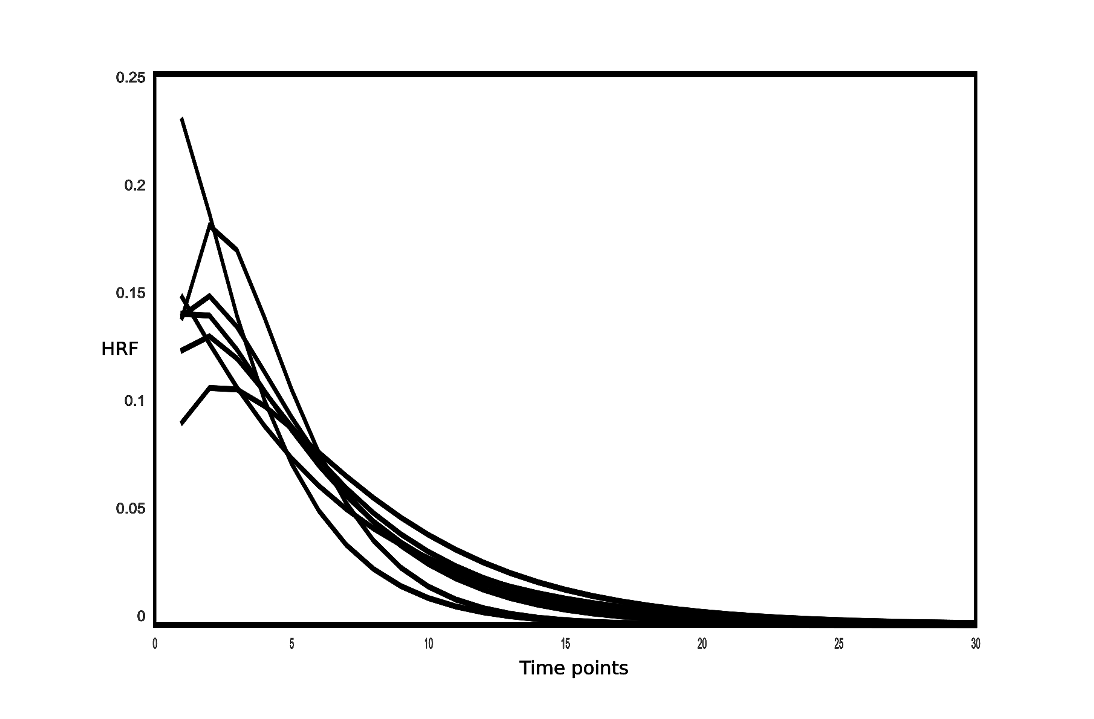
\includegraphics[width=\linewidth]{fig/encoding/gamma.eps}
	\caption{Comparison of haemodynamic response function learned by GAGamma encoding method for voxel 8 of subject 04847 across 7 different trials.}
	\label{fig:gamma}
\end{figure}


\subsubsection{Analysis of the Spike-train Encoded by GAGamma-16 Method}
Additionally, GAGamma-16 encoded spikes for the `seeing a picture', and the `reading a sentence' stimuli were independently analysed for interpreting the discriminating spatio-temporal influence of the spikes. As described earlier in the experimental protocol, the presentation of a certain stimulus within a trial follows an order, \emph{i.e.} for each stimuli class there exists subclasses of `presented first' or `presented second'. To analyse the effect of the first or second presentation of stimuli, the encoded dataset was separated into four classes, `picture presented first', `picture presented second', `sentence presented first' and `sentence presented second'. \figurenames \ref{fig:sub_04847} and \ref{fig:sub_07510} shows the comparison of the mean spike percentage across the trials for the four subclasses in subject 04847 and subject 07510. The points in the 3D plot correspond to the spatial location of the voxels. Each voxel belongs to two physiologically defined clusters or regions of interest, namely `CALC' and `LIPL.' The top row plots are the `picture' trials, and the bottom row trials are the `sentence' plots. The columns correspond to the stimulus (`picture' or `sentence') being presented first or second. The two clusters in each of the 3D plots relate to the two ROI's (top left is `LIPL' and bottom right is `CALC') of the brain structure. Functionally, the `CALC' region is responsible for central and peripheral vision whereas the `LIPL' region is related to visual attention. In both the subjects, `reading a sentence second' after `seeing a picture first' has more spike activity on average across the trials than the other way around, especially in the `LIPL' region. The mean spike activity in the `LIPL' is observed to be relatively higher ($0.59$ and $0.57$) when the subjects were `reading a sentence' than when the subjects were `seeing a picture' ($0.54$ and $0.55$). A two-sample T-test was conducted between the `seeing a picture' and the `reading a sentence' class in the `LIPL' region for the subjects to validate the previous result. The null hypothesis for the test conducted was the following, $H_0$: `there is no difference between the picture spike activity and sentence spike activity'. The null hypothesis was rejected at 5\% significance level with $p=5.27\times 10^{-18}$ for subject 04847 and with $p=7.05\times 10^{-12}$ for subject 07510. Hence, as per the T-test, the average spike activity across the trials over time for `seeing a picture' is significantly different from the average spike activity across trials over time for `reading a sentence'. Further, it must also be noted the sentences shown as part of the experiment are highly visual in nature (\emph{e.g.} `It is not true that the dollar is below the plus.') and requires a high image comprehension ability. This result is, therefore, consistent with the experimental results \citep{just2004imagery} obtained earlier which shows a greater degree of activation and functional connectivity in the `LIPL' region during cognitive tasks associated with high imagery sentence comprehension. This, in fact, also validates the ability of the proposed encoding algorithm to preserve the useful discriminatory information in the compressed encoded space of data.

\begin{sidewaysfigure}
	\subfloat[`seeing a picture' first during trial]{\label{fig:p11}
		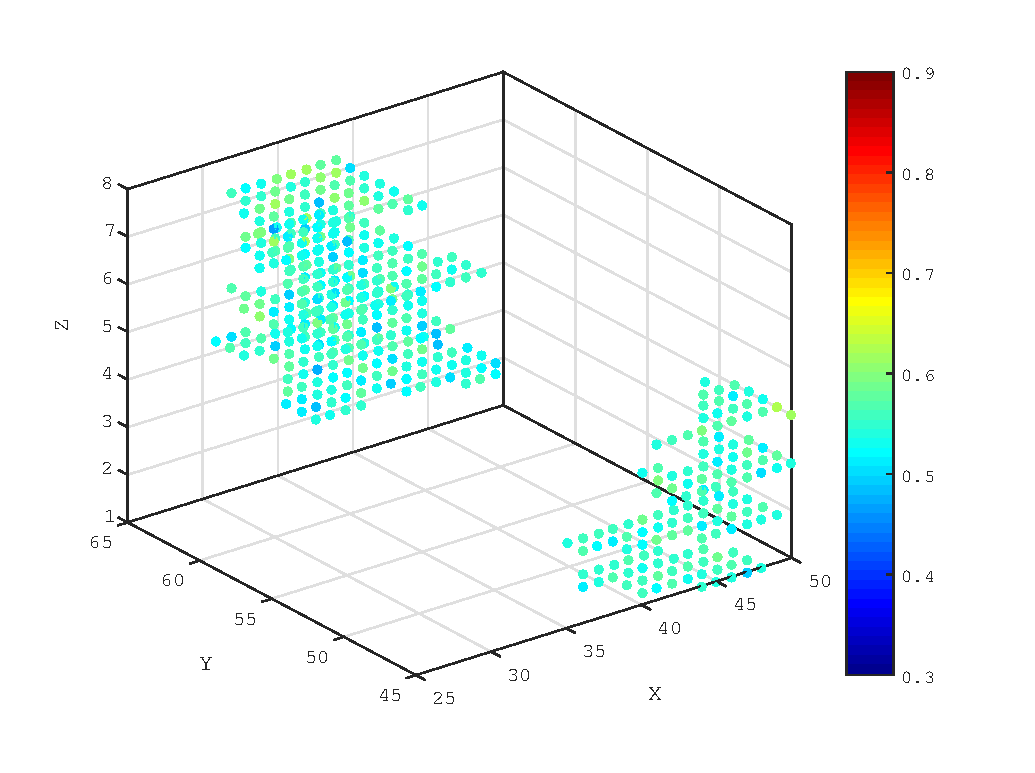
\includegraphics[width=0.42\textwidth]{fig/encoding/PICTURE_FIRST_04847.eps}}
	\subfloat[`seeing a picture' second during trial]{\label{fig:p12}
		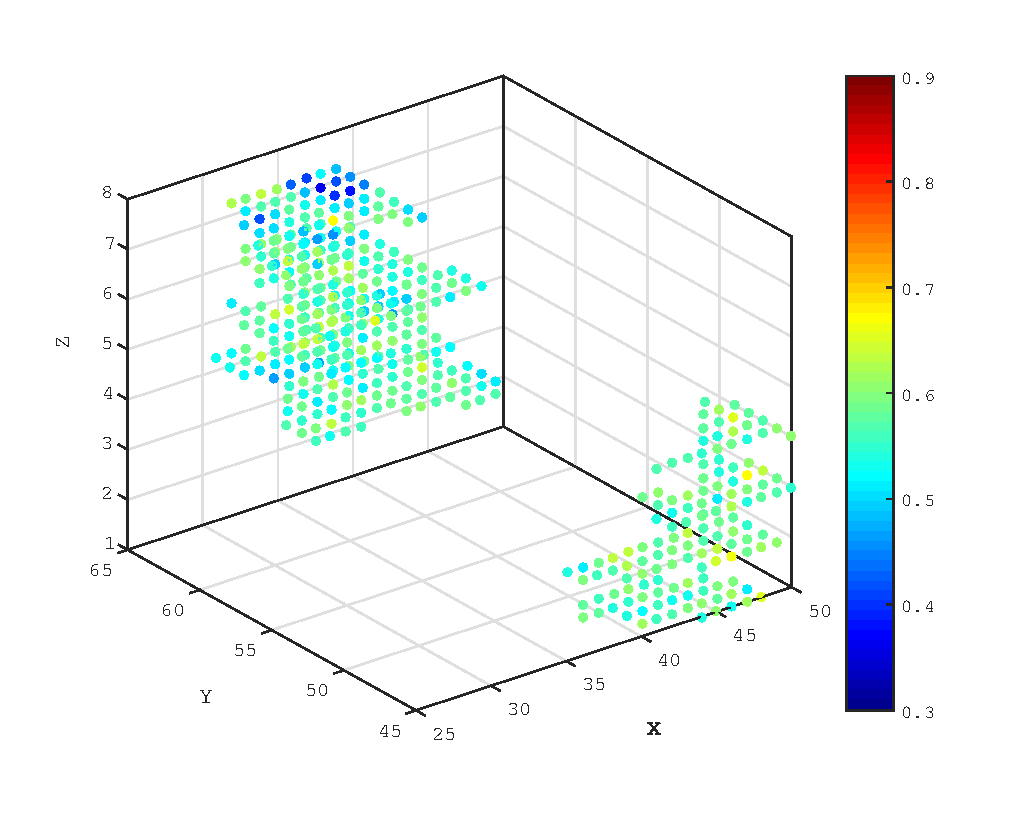
\includegraphics[width=0.42\textwidth]{fig/encoding/PICTURE_SECOND_04847.eps}}\\
	
	\subfloat[`reading a sentence' first during trial]{\label{fig:p13}
		\includegraphics[width=0.42\textwidth]{fig/encoding/SENTENCE_FIRST_04847.eps}}
	\subfloat[`reading a sentence' second during trial]{\label{fig:p14}
		\includegraphics[width=0.42\textwidth]{fig/encoding/SENTENCE_SECOND_04847.eps}}\\
	
	\caption{Comparative analysis of spike frequencies of the subject 04847 seeing picture vs. reading a sentence.}
	\label{fig:sub_04847}
\end{sidewaysfigure}

\begin{sidewaysfigure}
	\subfloat[`seeing a picture' first during trial]{\label{fig:p21}
		\includegraphics[width=0.42\textwidth]{fig/encoding/PICTURE_FIRST_07510.eps}}
	\subfloat[`seeing a picture' second during trial]{\label{fig:p22}
		\includegraphics[width=0.42\textwidth]{fig/encoding/PICTURE_SECOND_07510.eps}}\\
	
	\subfloat[`reading a sentence' first during trial]{\label{fig:p23}
		\includegraphics[width=0.42\textwidth]{fig/encoding/SENTENCE_FIRST_07510.eps}}
	\subfloat[`reading a sentence' second during trial]{\label{fig:p24}
		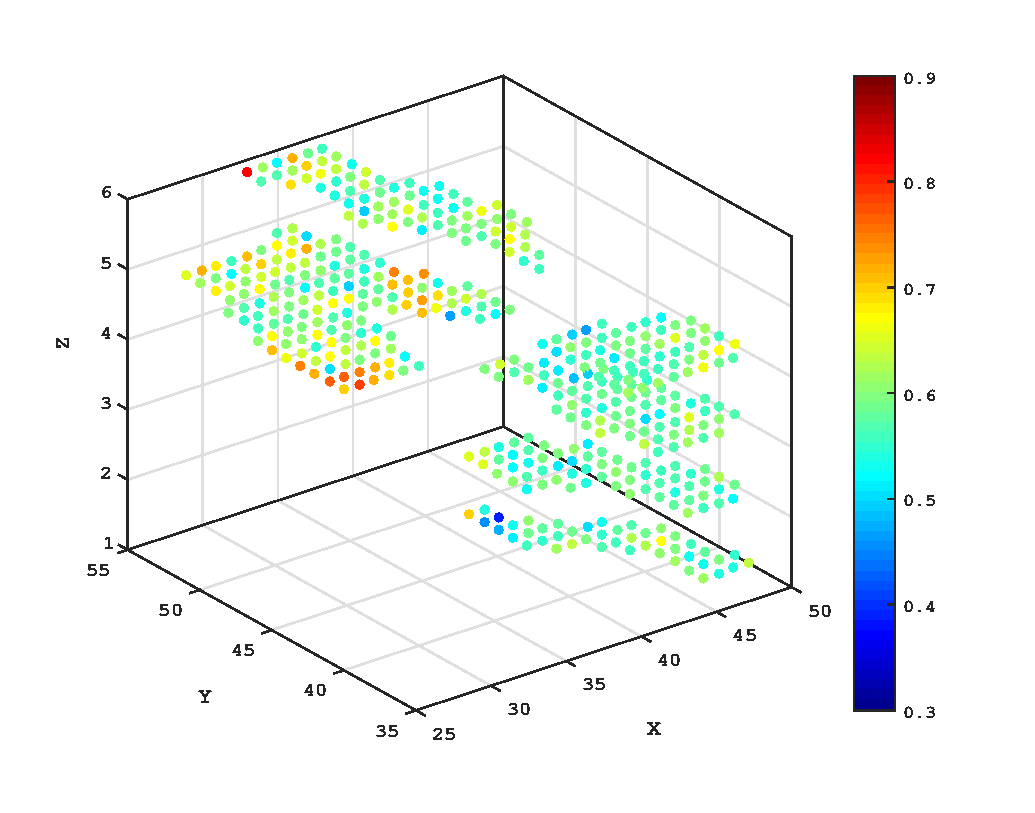
\includegraphics[width=0.42\textwidth]{fig/encoding/SENTENCE_SECOND_07510.eps}}\\
	
	\caption{Comparative analysis of spike frequencies of the subject 07510 seeing picture vs. reading a sentence.}
	\label{fig:sub_07510}
\end{sidewaysfigure}

% Please add the following required packages to your document preamble:
% \usepackage{booktabs}
\begin{table}
\centering
\caption{Average pairwise asynchronicity of three different voxels at the end of ten independent runs of GAGamma encoding.}
\label{tab:dist}
\begin{tabular}{@{}ccc@{}}
\toprule
\textbf{voxel ID} & $\mathbf{d_p}$ & $\mathbf{d_{vp}}$ \\ \midrule
$30$ & $24.18\pm 10.15$ & $0.23\pm 0.09$ \\
$468$ & $27.78\pm 11.96$ & $0.26\pm 0.10$ \\
$3429$ & $28.03\pm 11.31$ & $0.28\pm 0.11$ \\ \bottomrule
\end{tabular}
\end{table}

\tablename \ref{tab:dist} relates to the reproducibility of the spike-timings produced by the mixed integer genetic algorithm solver for the GAGamma encoding. The genetic algorithm being an evolutionary optimisation solver produces a non-reproducible result when on multiple iterations. Nevertheless, a pareto-optimal fitness value is guaranteed on each iteration. To validate the reliability of the GAGamma optimisation, in this instance, ten independent runs of GAGamma encoding was applied on three random voxels (30468 and 3429) from trial 12 of subject 04847. \tablename \ref{tab:dist} compares the similarity of the spike-trains produced by the GAGamma encoding using two spike-asynchronicity measures. They are the percentage asynchronicity $d_p$ and Victor Purpura distance $d_{vp}$ respectively. The Victor Purpura distance ($d_{vp}$) \citep{victor1997metric} metric is a cost based distance metric. The distance is defined by the minimum cost of converting one spike-train into the other using three operations: insertion (cost $1$); deletion (cost $1$); and shifting a spike by an interval $\delta t$ (cost $q|\delta t|$). For the smaller value of $q$ the distance metric approximates the spike count difference and hence supports rate coding. A higher penalty value of $q$, on the contrary, supports the number of non-coincidental spikes and hence temporal encoding. The comparison of the spike synchronicity using $d_p$ and $d_{vp}$ in \tablename \ref{tab:dist} shows that the spike-timings are correctly reproduced approximately $75\%$ of times.

\section{Summary and Conclusion}
In this Chapter, the focus was on using temporal encoding as a framework to concisely represent large volumes of data by spike-timings. By doing so, the existing discriminatory spatio-temporal information was preserved. In this regard, apart from using the existing temporal encoding techniques, a novel temporal encoding framework was formalised and a specific encoding algorithm for fMRI data, called GAGamma, was proposed. The experimental result on benchmark fMRI dataset shows the superiority of the temporal encoding algorithms, such as GAGamma and BSA, to succinctly represent the discriminatory information in the compressed encoded spike space without losing any appreciable amount of information. Thus, it achieves comparable or superior pattern recognition performance. It can be argued that the flexibility of the proposed encoding framework lies in its ability to inject known structure information about the data source and thus, provide the compression/encoding algorithms sufficient redundancy to represent the large dataset in an optimally concise manner. 

\pagebreak
\section{Contributions and Publications}
\begin{tcolorbox}[colback=black!5,colframe=black!40!black,title=Contributions]
	\begin{enumerate}
		\item A generalised \emph{a priori} knowledge driven optimisation framework for spike-time encoding of continuous data was formalised.  
		\item To elaborate the characteristics of this framework, a realisation of the proposed framework, namely GAGamma, was proposed for the purpose of encoding fMRI data using \emph{a priori} knowledge of the data source.
		\item The proposed encoding algorithm was applied and compared with state of the art encoding algorithms on a benchmark pattern recognition problem involving fMRI data. The results showed, in general, the uniqueness of the proposed temporal encoding framework not only lies in its ability to significantly compress the data, but also in keeping the discriminatory information intact, which is extremely useful for pattern recognition tasks. 
	\end{enumerate}
	
\end{tcolorbox}

\begin{tcolorbox}[colback=black!5,colframe=black!40!black,title=Publications]
	\begin{enumerate}
		\item \textbf{Sengupta, N.}, \& Kasabov, N. (2017). Spike-time encoding as a data compression technique for pattern recognition of temporal data. Information Sciences,  406, 133-145.	
		
		\item \textbf{Sengupta, N.}, Scott, N., \& Kasabov, N. (2015). Framework for knowledge driven optimisation based data encoding for brain data modelling using spiking neural network architecture. In Proceedings of the Fifth International Conference on Fuzzy and Neuro Computing (FANCCO-2015) (pp. 109-118). Springer, Cham.
	\end{enumerate}
\end{tcolorbox}